\section{Evolution and Structure of Content Delivery Networks}\label{sec:aslevel:background}

This section describes the background on traffic exchange among ISPs and CDNs and presents related work.
We start with an introduction in ISP relations and charging models.
We provide the basic ideas of content delivery network structures and their evolution.
%Finally, we introduce studies that infer the inter-AS relations based on BGP routing information.
We briefly describe the structure of the YouTube video CDN.
Finally we evaluate the Internet Census Dataset to assess the potential of peer assisted CDNs.

\subsection{ISP Relations and Charging Models}

%Autonomous systems are individual parts of the Internet, which are operated by ISPs.
On a technical level, the traffic exchange between ASs is controlled by the Border Gateway Protocol (BGP)~\cite{trangia2009}. Commercial relations between ISPs determine the routing policies configured via BGP.
%The traffic exchanged between autonomous systems is inter-domain traffic. It is differentiated from intra-domain traffic, which is the traffic in the autonomous system.

An ISP must buy transit services to access parts of the Internet it neither owns nor can access by its customers.
Hence, to route traffic between ASs, ISPs engage in business relationships.
These business relationships are usually not open for public but they can be abstracted into three common types \cite{gao2001}.
The relationship between two ASs can be transit, peering or sibling.
A transit link is present if the customer AS pays the provider AS for transit service, i.e., the provider forwards the traffic of the customer and its customers.
In peering relations the ASs have an agreement that they exchange each others traffic and the traffic of their customers, without paying each other.
Sibling links between ASs of the same organization. These relations are defined in business agreements and kept secret, but they can be inferred by analyzing the routing between autonomous systems.

As peering links and sibling links are the same in terms of money flow, we consider sibling links as peering links in this manuscript. For the same reason most datasets available do not contain sibling links.
Hence, we only consider transit and peering inter-domain links from now on.
\reffig{fig:aslevel:p2pcdn} shows AS topologies with ASs interconnected with inter-domain links.
%Inter-AS links are either peering links or transit links.

\subsection{Evolution of Content Delivery Networks}
% The drawback of client-server architectures for content distribution is their limited scalability.
% -> P2P, legal issues, coordination

%The two most popular solutions to this problem are content delivery concepts that work according to the P2P or CDN principle.

Host-to-host
ALTO

Host-to-content Information Centric Networking (ICN)

While the amount of traffic transported over P2P networks remained about the same, the traffic transported by CDNs has increased exponentially \cite{cisco2016} in the last years.
The number of users watching videos on demand has massively increased and the bandwidth to access videos is much higher.
Furthermore, the increased bandwidth enables web services to be interactive by using dynamic server- or client-side scripts.
The appearance of dynamic services and the increasing quality of multimedia content raises user expectations and the demand on the servers.
To bring content in high quality to end-users with low latency and to deal with increasing demand, content providers have to replicate and distribute the content on caches to get it close to end-users.
Hence, in CDNs, c.f., \reffig{fig:aslevel:cdn}, the storage resources are managed data centers or caches.
%Thus, content delivery infrastructures such as the Google CDN evolved.
%The largest amount of traffic is now transported by CDNs.

% \begin{table}
% 	\caption{P2PvsCDN}
% \end{table}

%To understand why distributed measurements are necessary and to provide the basic ideas of content delivery network structures, we briefly describe the evolution of content delivery networks and the functionality of the YouTube CDN.
%Since the launch of the YouTube service, content delivery has drastically changed.

\begin{figure}[bt]
	\centering
\vspace{-0.2cm}
\hspace{-0.5cm}
	\begin{subfigure}[b]{0.54\textwidth}
	  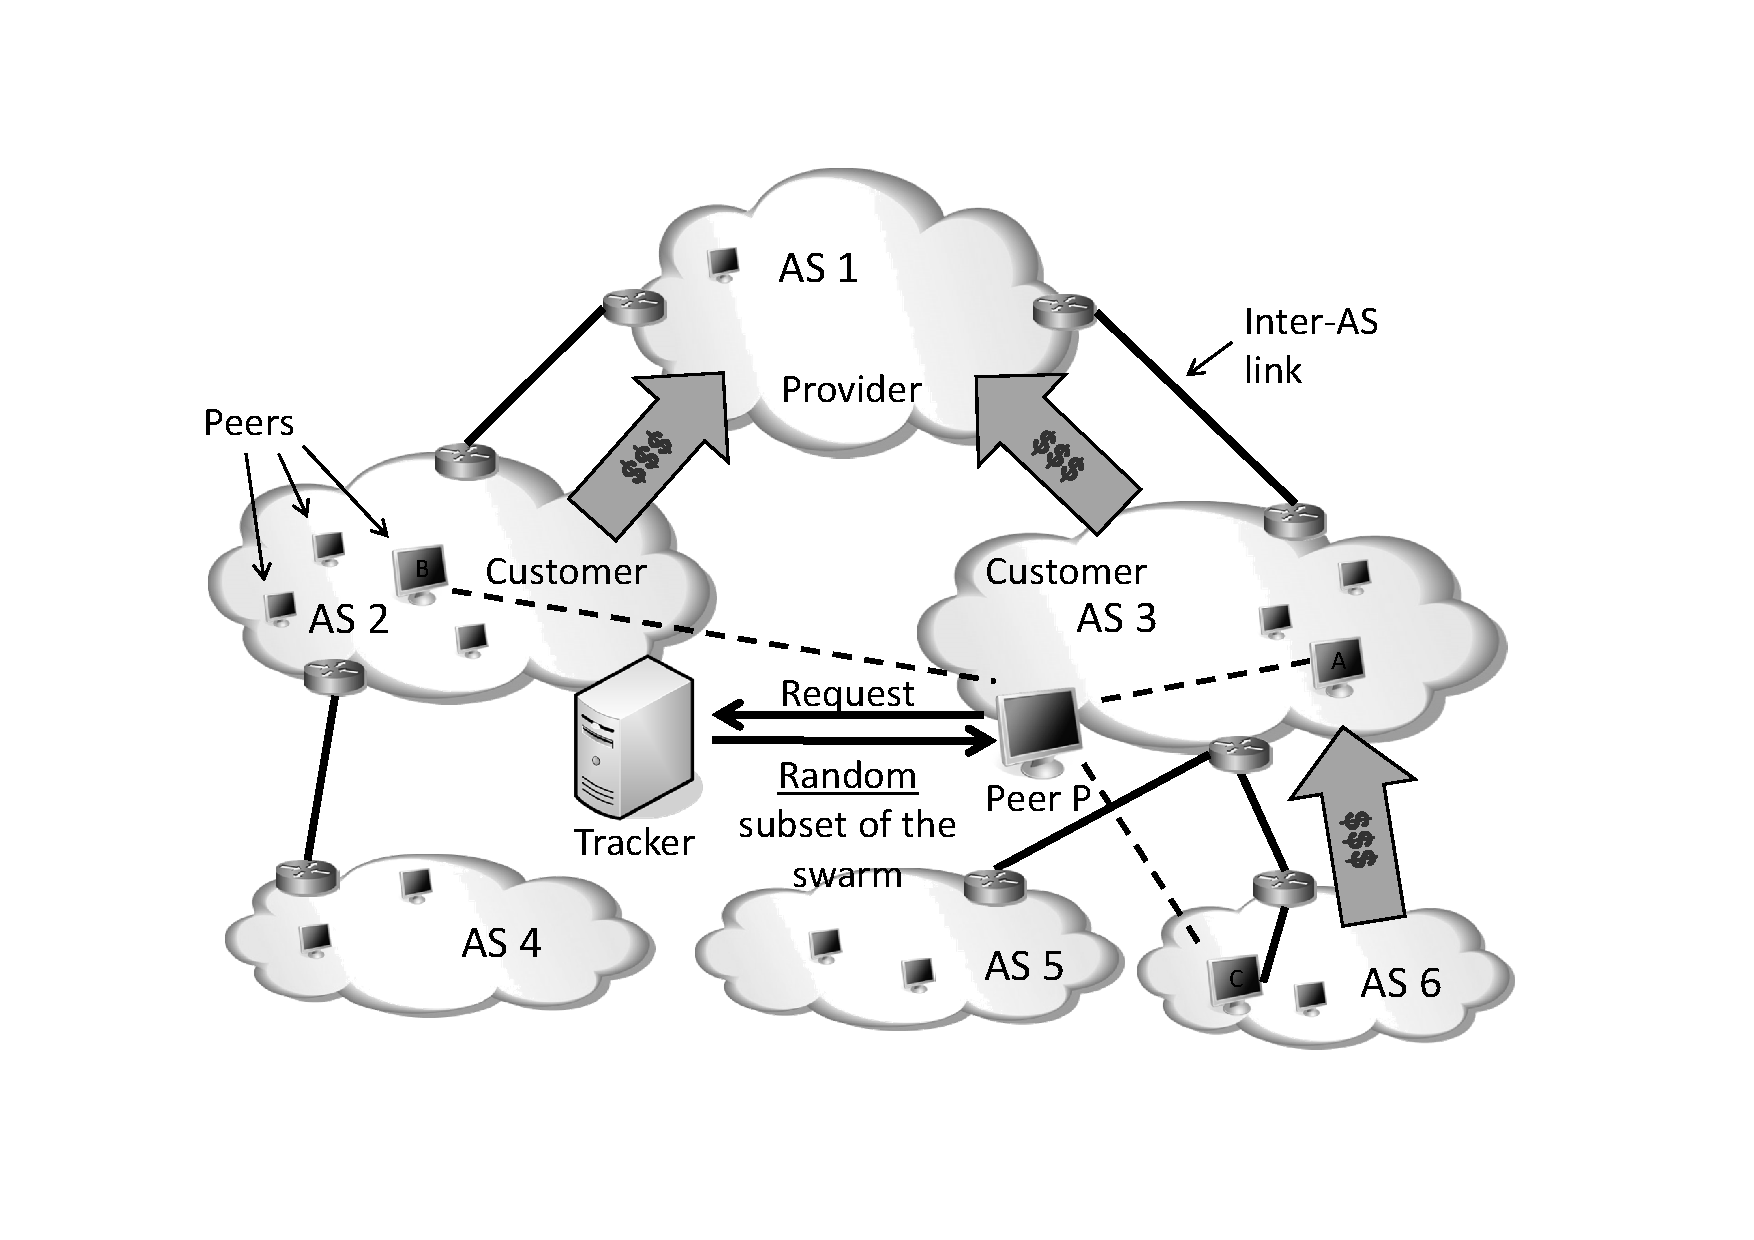
\includegraphics[width=\textwidth]{aslevel/figs/p2p}
    \vspace{-0.5cm}
    \caption{P2P network}
    \label{fig:aslevel:p2p}
  \end{subfigure}
\hspace{-0.5cm}
	\begin{subfigure}[b]{0.54\textwidth}
	 	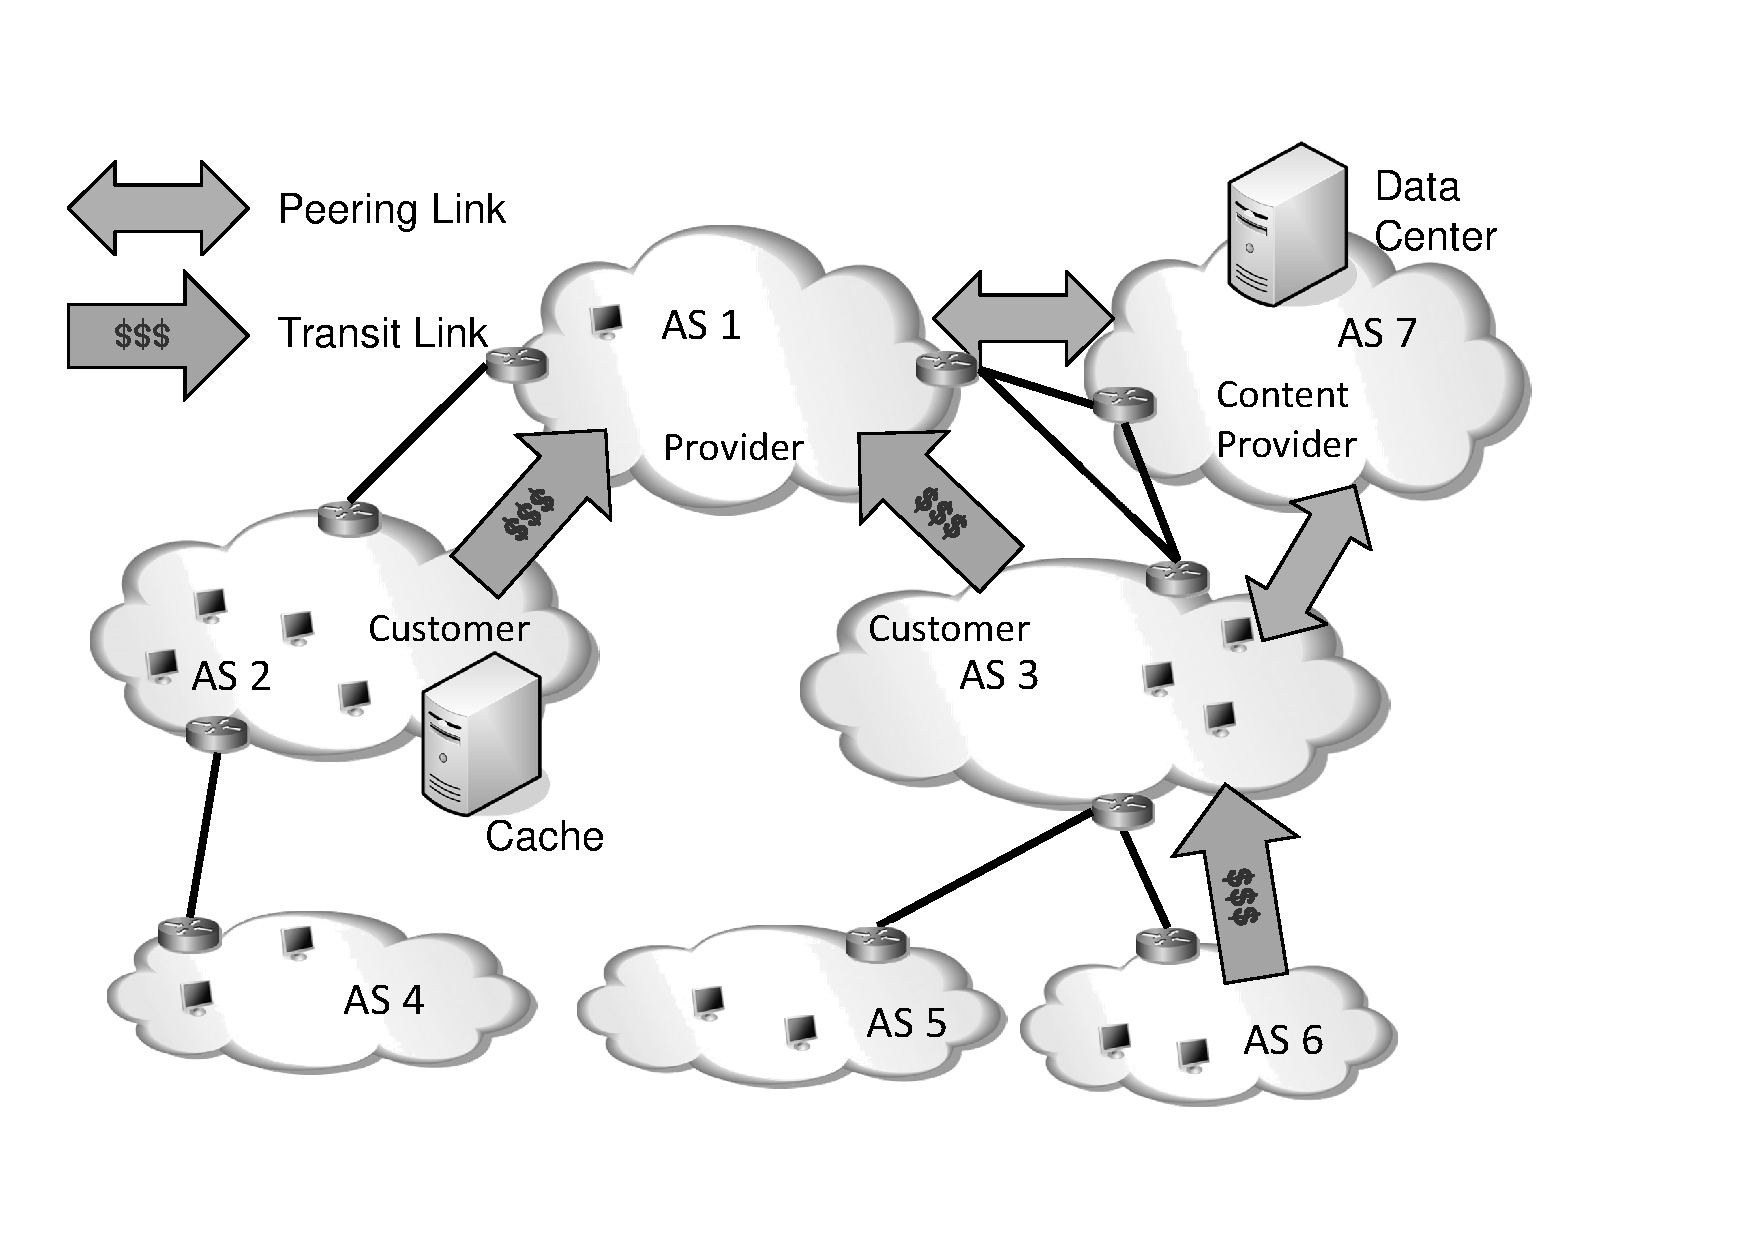
\includegraphics[width=\textwidth]{aslevel/figs/cdn}
    \vspace{-0.5cm}
    \caption{Content delivery network}
    \label{fig:aslevel:cdn}
	\end{subfigure}
\hspace{-0.5cm}
	\caption{Autonomous system topology with a P2P network (left) and a CDN (right).}\label{fig:aslevel:p2pcdn}
\end{figure}

The global expansion of the CDNs also changes the structure of the Internet.
Google has set up a global backbone which interconnects Google's data centers to important edge points of presence.
Since these points of presence are distributed across the globe, Google can offer direct peering links to access networks with many end users, c.f. AS 3 and AS 7 in \reffig{fig:aslevel:cdn}.
Such, access network providers save transit costs, while Google is able to offer services with low latency.
To bring content even closer to users, ISPs can deploy Google cache servers inside their own network to serve popular content, including YouTube videos~\cite{gcc}.

To select the closest server for a content request and to implement load balancing, CDNs use the Domain Name System (DNS).
Typically a user watches a YouTube video by visiting a YouTube video URL with a web browser.
The browser then contacts the local DNS server to resolve the hostname.
Thereafter, the HTTP request is directed to a front end web server that returns an HTML page including URLs for default and fallback video servers.
These URLs are again resolved by DNS servers to physical video servers, which stream the content.
The last DNS resolution can happen repeatedly until a server with enough capacity is found to serve the request.
Thus, load balancing between the servers is achieved~\cite{adhikari2012vivisecting}.

The next generation of content delivery networks try to bring content even closer to users by using resources in home networks or mobile network cells for caching.
A recent approach \cite{valancius2009greening} proposes to augment spare capacities on customer premise equipment (CPE) such as home routers to assist content delivery, showing that there is a high potential to save energy, although the capacity of home routers is small and the uplink is limited.
The content is transported locally in a P2P manner keeping the traffic within the AS.
Another example are femto caching architectures \cite{golrezaei2013femtocaching}, where content is cached on femto-basestations with small capacity but with considerable storage space.
The potential of these approaches highly depends on the number of caches available and their capacity for content delivery.
In order to assess the number of home routers available in an AS, which can be equipped with caches, we characterize the Internet subscriptions on AS Level.

% \subsection{Structure of Global Content Delivery Network}
%
% CDNs aim to to deliver services with high performance, high reliability, and low latency for users.
% The network infrastructure of global CDNs has three distinct elements, the core data centers, edge points of presence (PoPs) and edge caches to exchange traffic efficiently and cost-effectively.

\subsection{Characterization of Internet Subscriptions on AS Level}\label{sec:aslevel:census}

The performance of systems using CPE or resources provided by end-users depends on the capacity and number of devices available.
To assess the potential of a CDN, which uses the home routers provided with Internet subscriptions as caches, the number of active subscribers in an AS has to be known.
Hence, the goal is to identify the number of home routers with active Internet subscriptions in each AS.
Assuming that the number of active IP-addresses is correlated to the number of subscribers in an AS, we use the Internet Census Dataset to determine the distribution of active IP-addresses on ASs.

We use the Internet Census Dataset \cite{carna2013} to determine the number of active IP-addresses for each AS in the Internet.
The Internet Census Dataset provides a scan on the active IP-addresses in the Internet based on a full probing of the entire IPv4 Internet.
%The Internet Census Dataset\cite{carna2013} was conducted from June to October 2012.
The scan was conducted from June to October 2012 by infecting several hundred thousand unprotected devices on the Internet to form the so called \emph{carna} botnet.
The botnet functioned as distributed port scanner that transfered the results to a central server.

%The complete IPv4-address room was scanned using a bot-net consisting of 4,200,000 nodes.
In the ICMP ping scan more than 420 million replied to requests more than once.
The service probe data reveals open ports on devices which is used to infer the type of device.
The Internet Census Dataset was validated forensically in \cite{dainotticaida} by aligning the probes of the botnet with the traffic captured at the UCSD Network Telescope\footnote{\url{https://www.caida.org/projects/network_telescope/}}, which is a large darknet, i.e., IP addresses that are inactive, thus not accepting connections.
The raw logs of the carna botnet erroneously reported that a large number of IPs in the darknet were active, likely due to the presence of HTTP proxies.
However, according to \cite{dainotticaida}, only about 3\% of the host probe and port scan logs are potentially affected by this problem.
Unaffected by this issue are the logs based on ICMP pings and actual responses from the target hosts, which are used in our study.
In \cite{krenc2014internet} the scope of the dataset is taken into perspective and show that, although there are some qualitative problems, the measurement data seems to be authentic.
%We use the Internet Census Dataset to determine the number of active IP-addresses for each autonomous system in the Internet.

We use an IP to ASN mapping to derive the autonomous system number for each IP-address. There are different services, that provide an IP to ASN mapping.
The whois-service can be used to get the current ASN for an IP-address.
To enable an efficient evaluation we used the MAXMIND GeoLite ASN database \cite{geo_ip}, which is updated every month and can be downloaded and used as a local database.
The results of the MAXMIND GeoLite ASN database were cross checked with results obtained from whois, which showed no differences.

The ICMP ping scan discovered a total of 598,180,914 IP-addresses.
The service probe scan discovered 244,000 IP-addresses that listen to port 9100 and are identified as print servers, and 70.84 million IP-addresses of web-servers that listen to port 80.
Assuming that most network functions do not reply to ICMP ping requests and neglecting different network functions, this results in 88.1\% of IP-addresses assigned to end-user devices.
Since the Internet Census the number of Internet users increased, which also has to be considered.
According to \cite{itu2015facts} there is a 7\% annual increase in fixed-broadband subscriptions in the past three years.
%From 2012 to 2014 the number of Internet users increased by almost 500,000,000 according to \cite{•}.

% \begin{figure}[tb]
% \centering
% 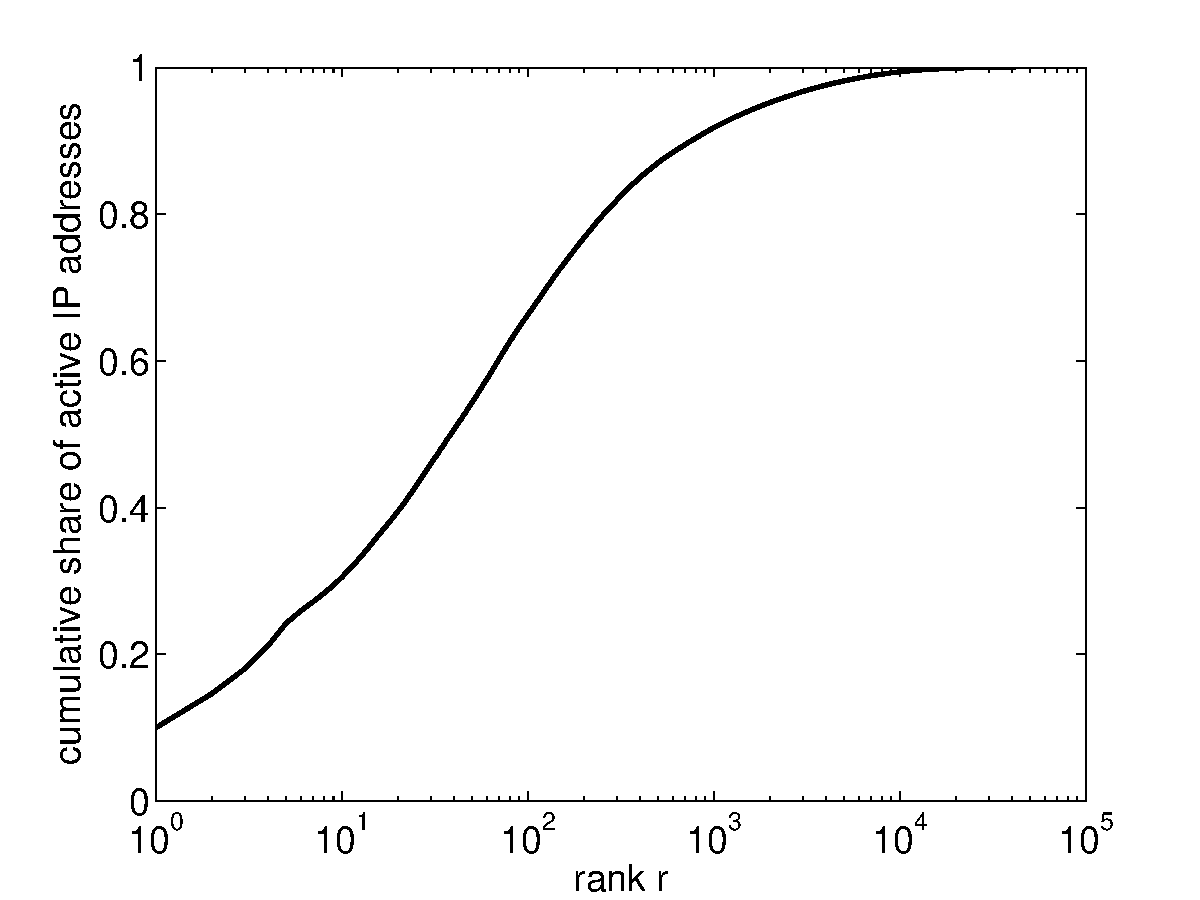
\includegraphics[width=0.49\textwidth]{aslevel/census/figs/shareactiveIPs}
% \caption{Cumulative share of active IP-addresses in autonmous systems ranked in descending order.}
% \label{fig:shareactiveIPs}
% \end{figure}
%
% \begin{figure}[tb]
% \centering
% 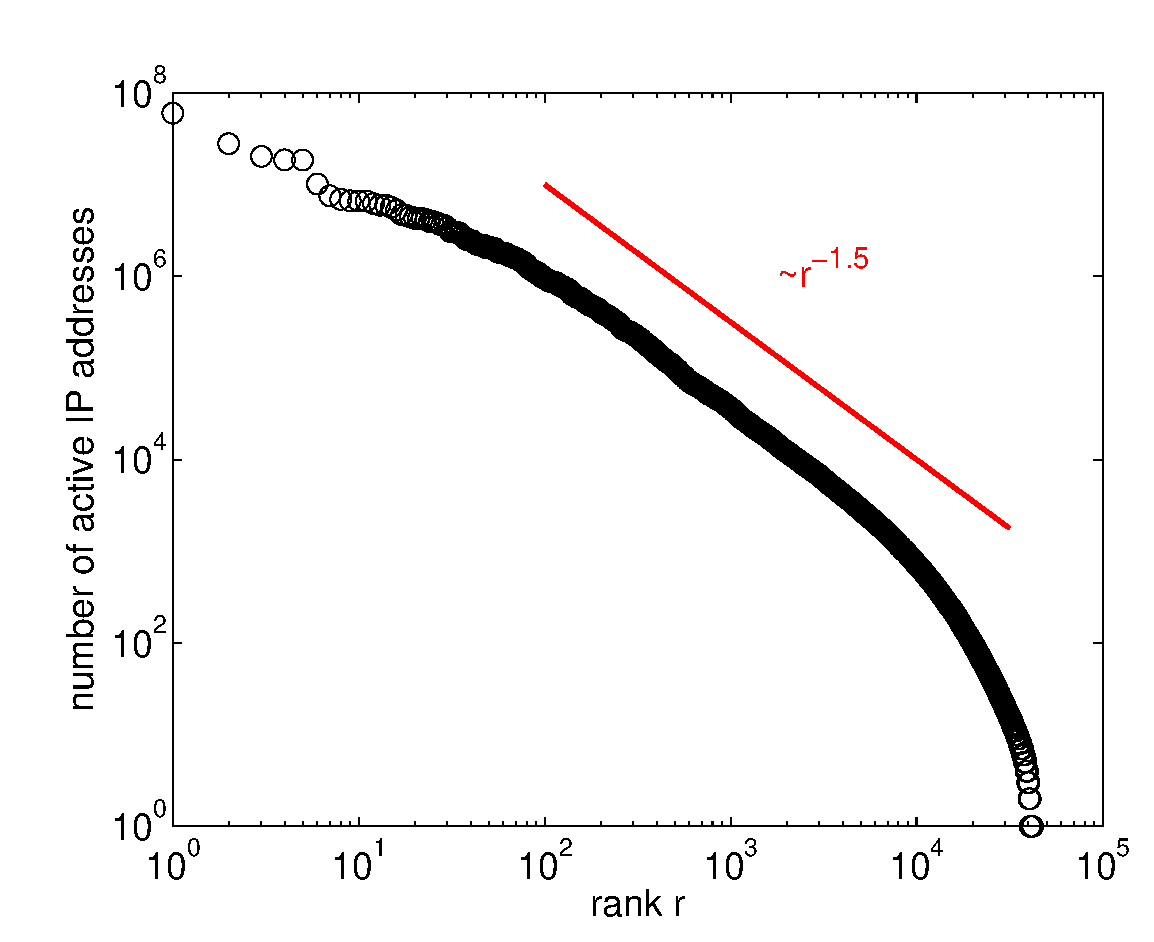
\includegraphics[width=0.49\textwidth]{aslevel/census/figs/activeIPs}
% \caption{Rank of Internet providers with number of active IP-addresses per AS.}
% \label{fig:asrank}
% \end{figure}

\begin{figure*}[bt]
\begin{minipage}[b]{0.49\textwidth}
  \centering
  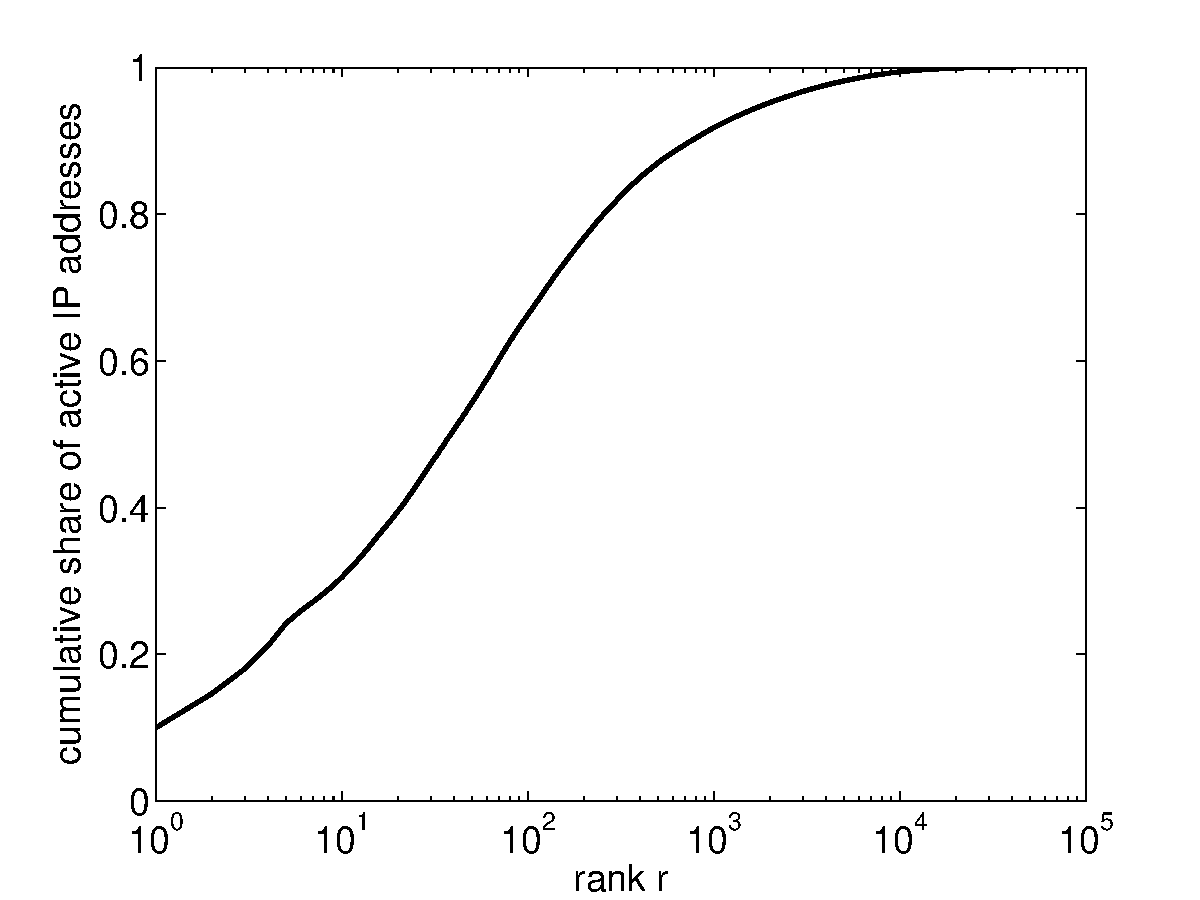
\includegraphics[width=1\textwidth]{aslevel/census/figs/shareactiveIPs}
  \caption{Cumulative share of active IPs in autonmous systems ranked in descending order.}
  \label{fig:shareactiveIPs}
\end{minipage}
\hspace{0.01\textwidth}
\begin{minipage}[b]{0.49\textwidth}
  \centering
  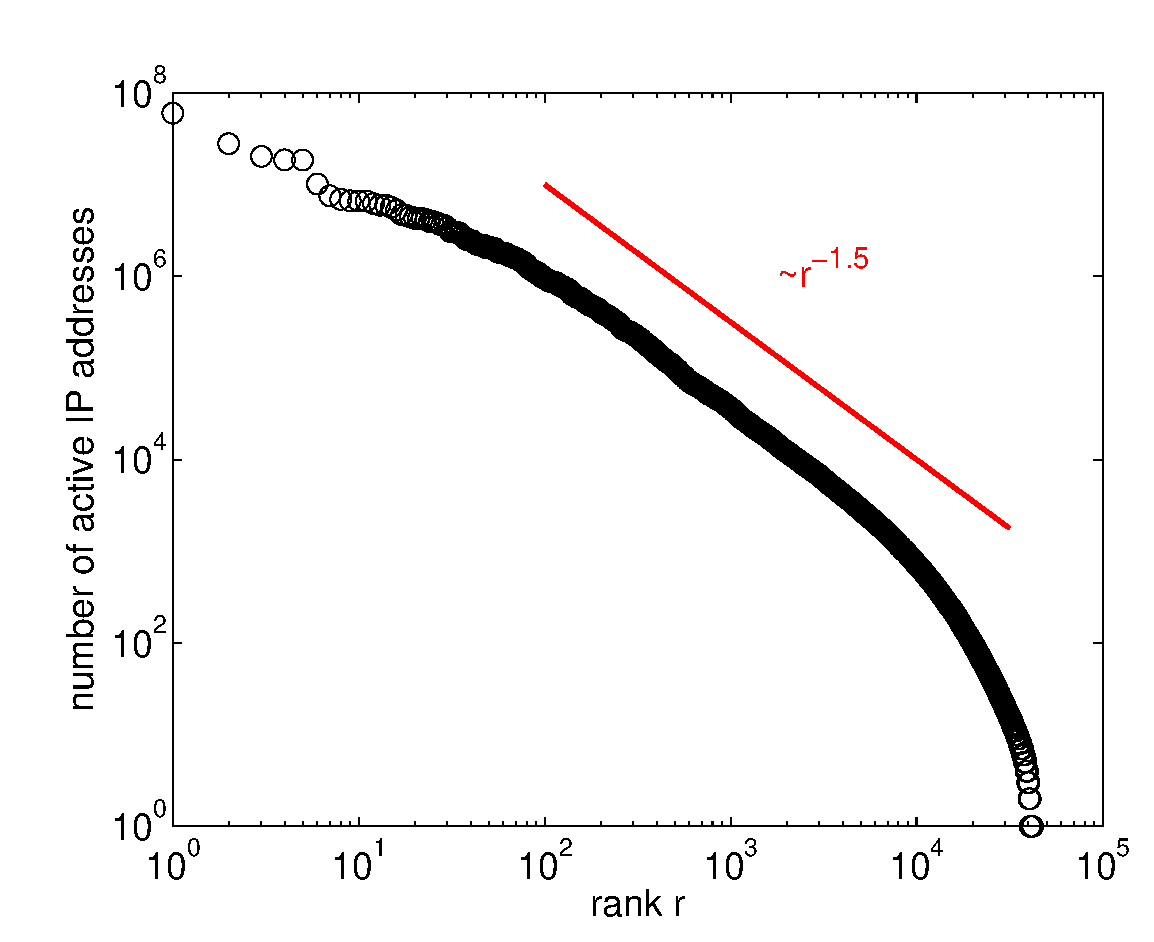
\includegraphics[width=\textwidth]{aslevel/census/figs/activeIPs}
  \caption{Rank of Internet providers with number of active IPs per AS.}
  \label{fig:asrank}
\end{minipage}
\end{figure*}

\reffig{fig:shareactiveIPs} shows the cumulative share of active IP-addresses in the autonomous systems ranked in descending order.
The 100 largest autonomous systems make up 2/3 of active IPs and more than 85\% of the IPs are active in only 1\% of the autonomous systems. The 10 largest autonomous systems already contain 30\% of the active IPs.

\reffig{fig:asrank} shows the number of active IP-addresses per AS ranked in descending order.
The top 5 ASs are shown in table~\ref{tab:asrank}.
The AS with most active IP-addresses is ChinaTelecom with almost 60 million active IPs, followed by another Chinese provider.
The largest AS in the US is Comcast on rank three.
The largest Korean and German providers are ranked 4 and 5 with more than 18 million active IPs.
The number of active IP addresses can be approximated with a power law with slope 1.5 that drops a little for low ranks.
This shows that the distribution of active IP addresses on ASs is highly heterogeneous.
That means the potential of approaches leveraging spare resources on home routers highly depends on the AS.

\begin{table}[tb]
\centering
\caption{Rank of top 5 provider with most active IP-addresses.}
\label{tab:asrank}
\begin{tabular}{|c|c|c|c|}
\hline
rank r & ASN & provider & \# active IPs  \\
\hline
1 & 4134 & ChinaTelecom & 59,824,824 \\
2 & 4837 & China-Network-Communication-Group & 27,776,643 \\
3 & 7922 & Comcast & 20,227,918 \\
4 & 4766 & KoreaTelecom & 18,502,963 \\
5 & 3320 & DeutscheTelekomAG & 18,476,519 \\
\hline
\end{tabular}
\end{table}
